\documentclass[11pt]{article}

\usepackage{latexsym}
\usepackage{amsmath}
\usepackage{amssymb}
\usepackage{amsthm}
\usepackage{graphicx}
\usepackage{wrapfig}
\usepackage{pseudocode}
\usepackage{url}
\usepackage[backref, colorlinks=true, citecolor=red, urlcolor=blue, pdfauthor={Jyh-Ming Lien}]{hyperref}


\newcommand{\handout}[5]{
  \noindent
  \begin{center}
  \framebox{
    \vbox{
      \hbox to 5.78in { {\bf } \hfill #2 }
      \vspace{4mm}
      \hbox to 5.78in { {\Large \hfill #5  \hfill} }
      \vspace{2mm}
      \hbox to 5.78in { {\em #3 \hfill #4} }
    }
  }
  \end{center}
  \vspace*{4mm}
}

\newcommand{\lecture}[4]{\handout{#1}{#2}{#3}{}{Report for #1}}

\newtheorem{theorem}{Theorem}
\newtheorem{corollary}[theorem]{Corollary}
\newtheorem{lemma}[theorem]{Lemma}
\newtheorem{observation}[theorem]{Observation}
\newtheorem{proposition}[theorem]{Proposition}
\newtheorem{definition}[theorem]{Definition}
\newtheorem{claim}[theorem]{Claim}
\newtheorem{fact}[theorem]{Fact}
\newtheorem{assumption}[theorem]{Assumption}

% 1-inch margins, from fullpage.sty by H.Partl, Version 2, Dec. 15, 1988.
\topmargin 0pt
\advance \topmargin by -\headheight
\advance \topmargin by -\headsep
\textheight 8.9in
\oddsidemargin 0pt
\evensidemargin \oddsidemargin
\marginparwidth 0.5in
\textwidth 6.5in

\parindent 0in
\parskip 1.5ex
%\renewcommand{\baselinestretch}{1.25}

\begin{document}

\lecture{Advance Algorithm Programming Assignment 1 Part3 }{Fall 2015}{Moran Kim}


\section{Implementation Details}
The crust algorithm is constructed for surface reconstruction of given scattered data in $\mathbb{R}^d$. The idea of the crust of a set of points is a set of triangles(in 3D) whose circumsphere is empty of input points. In 2-dimensional case the vertices of the Voronoi diagram of a dense sample approximate the medial axis. But, in 3D this is not true. We need to use the "poles" of the voronoi cells. The pole has two kinds. One is 'positive pole' and the other is 'negative pole'. If a data point is an interior point, we call the farthest voronoi vertex as a positive pole. If a site is on the convex hull of given data point set, the positive pole is undefined. Instead, we define a negative pole using the normal direction(the average of the outer normals of the adjacent triangles.) which is the voronoi vertex withe negative projection on the normal vector that is farthest from the site. After computing all the pole from given data. We compute the Delauany triangulation of the given data and computed poles. For the detailed implementation you can check the reference in the code. To compute the pole which is a voronoi vertex, we need a loop that circulate set of facet. Instead circulating the set of vertices in each facet. Given a site, to get a farthest voronoi vertex we need to go round every neighbor facet and check whether their voronoi vertices are the farthest one. In most cases, to deal this surface reconstruction problem simple, I used index of facets and vertices instead dealing directly with the data.
\section{Example Output}
I tried the cube, bunny, ellipsoid and bb which has holes in their triangulated surface. The problem happens because the data have sampling weakness. And also I think the poles which are so far from the data points or so close to data points make the situation worse. To deal with these kind of poles, I can put some restriction about the computed poles. For example, first computing the maximum distance of the given data points. If the distance of the pole and corresponding site of the pole is greater than some constant times the maximum distance of the given data points. We can exclude that kind of weird poles. I didn't implemented this part since I am out of time, but I will try to add this part later.

\begin{figure}[h]
  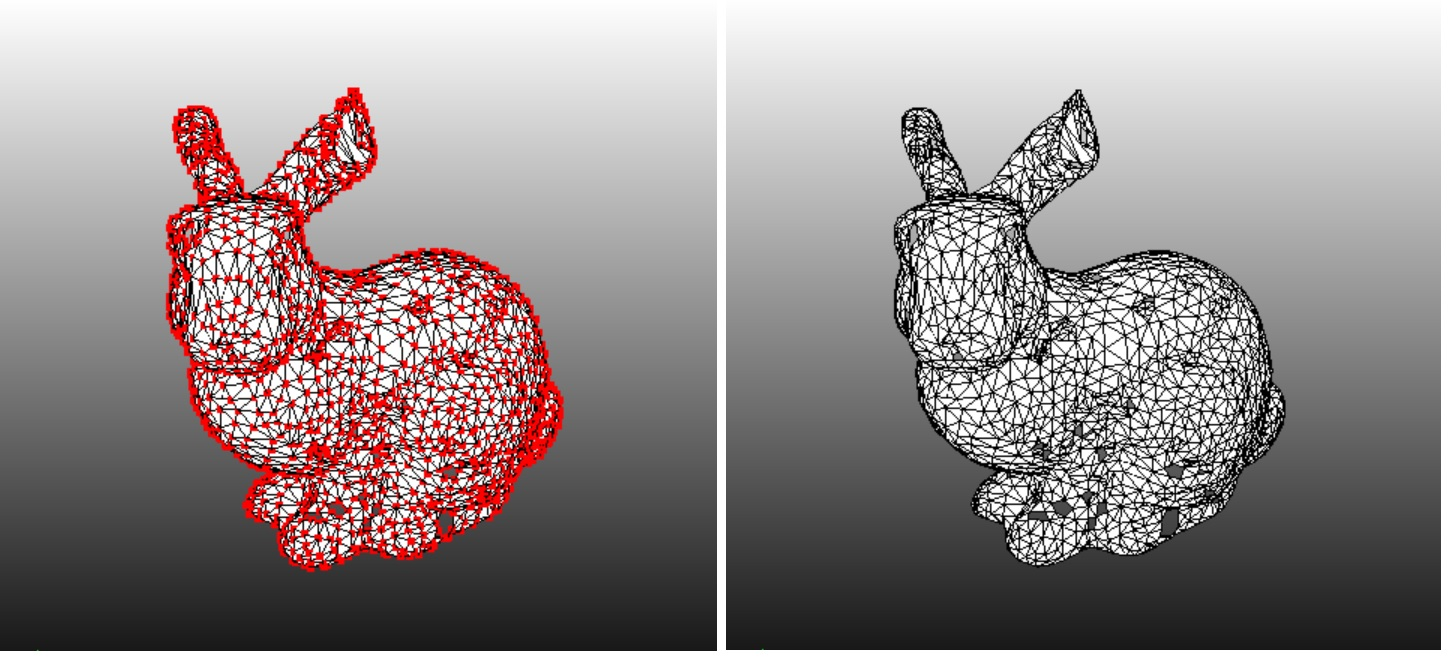
\includegraphics[width=120mm]{crust_bunny.jpg}\\
  Fig 1. Triangulated surface of bunny has some holes.
\end{figure}

\begin{figure}[h]
  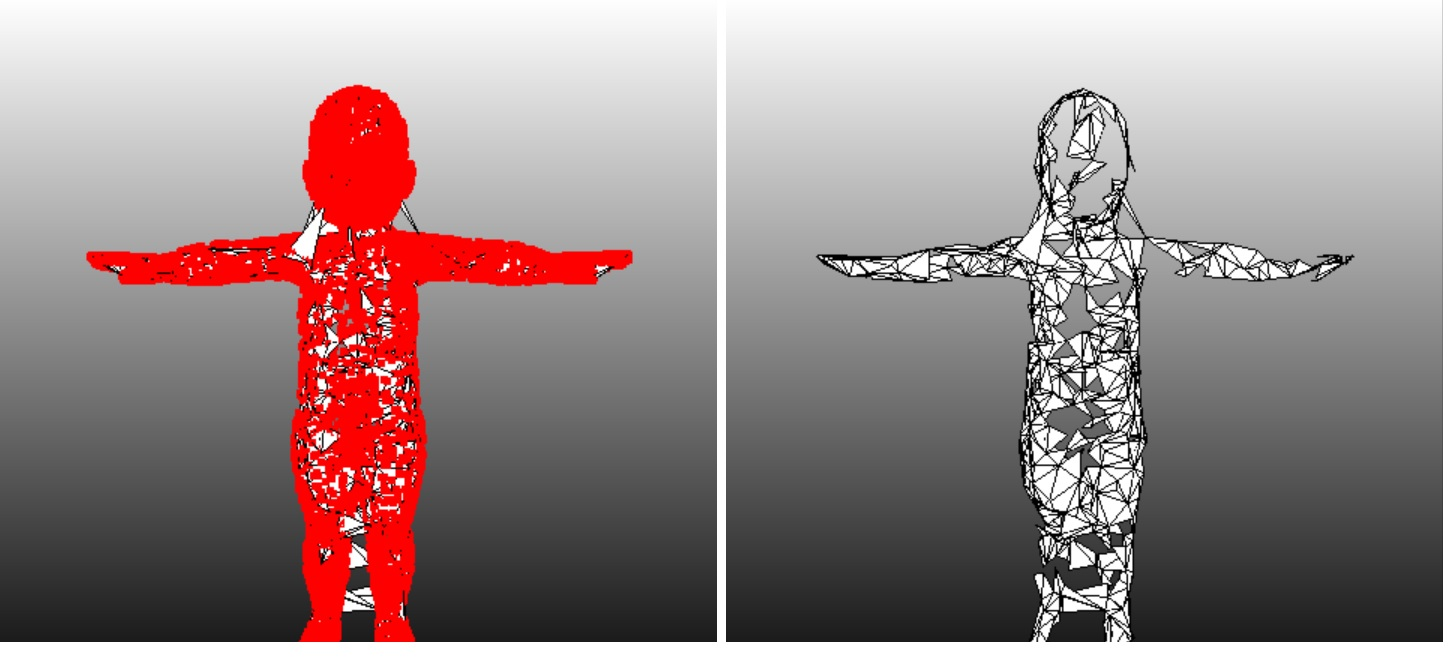
\includegraphics[width=120mm]{crust_bb.jpg}\\
  Fig 2. Triangulate surface of a human. In the foot part, maybe some poles are close to data points. 
\end{figure}


\begin{figure}[h]
  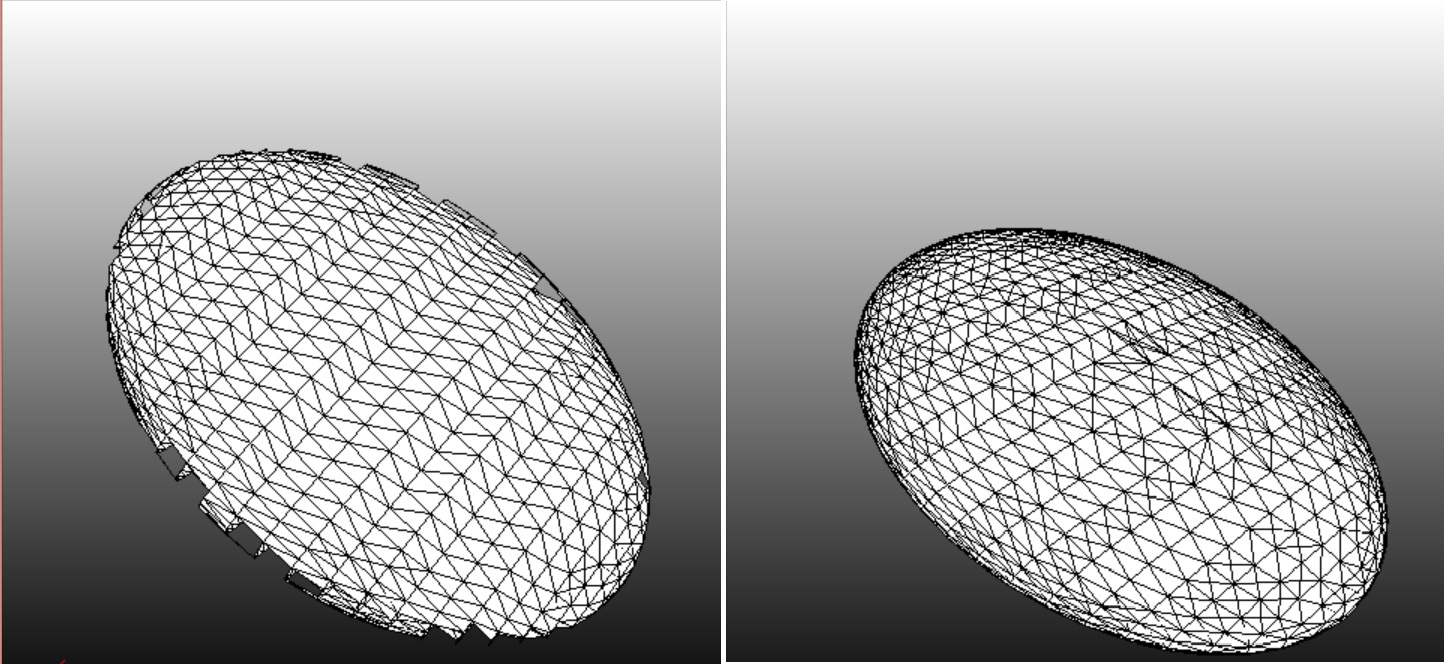
\includegraphics[width=120mm]{crust_ellipsoid.jpg}\\
  Fig 3. Triangulated surface of ellipsoid using crust algorithm(left), and delauany triagulation(right).
\end{figure}



\section{Known bugs/limitations}
As I mentioned above in the pictures I got have some holes in there triangulated surface. I think I need to exclude the poles which are really far from the data points. And the poles which are too close to the data points also make the triangulation bad. When I tried the cube data, I got a cube with only 5 faces(triangulated face). If the code was correct this should produce a picture with 6 faces. I am linger on it.  

\begin{figure}[h]
  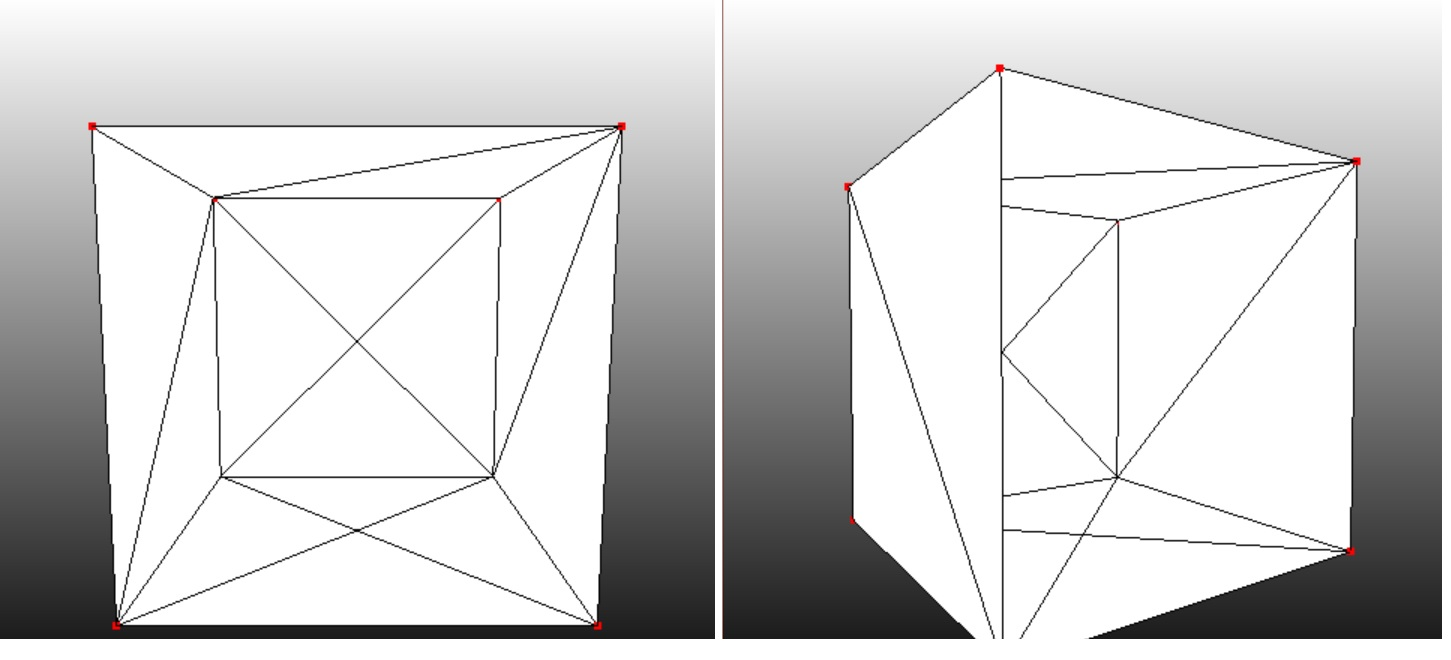
\includegraphics[width=120mm]{crust_cube.jpg}\\
  Fig 4. The triangulated surface of cube has only five faces. 
\end{figure}

\bibliographystyle{plain}
\bibliography{report}

\end{document}


